
\usetikzlibrary{positioning,arrows.meta,quotes}
\usetikzlibrary{shapes,snakes}
\usetikzlibrary{bayesnet}
\tikzset{>=latex}
\tikzstyle{plate caption} = [caption, node distance=0, inner sep=0pt,
below left=5pt and 0pt of #1.south]
 

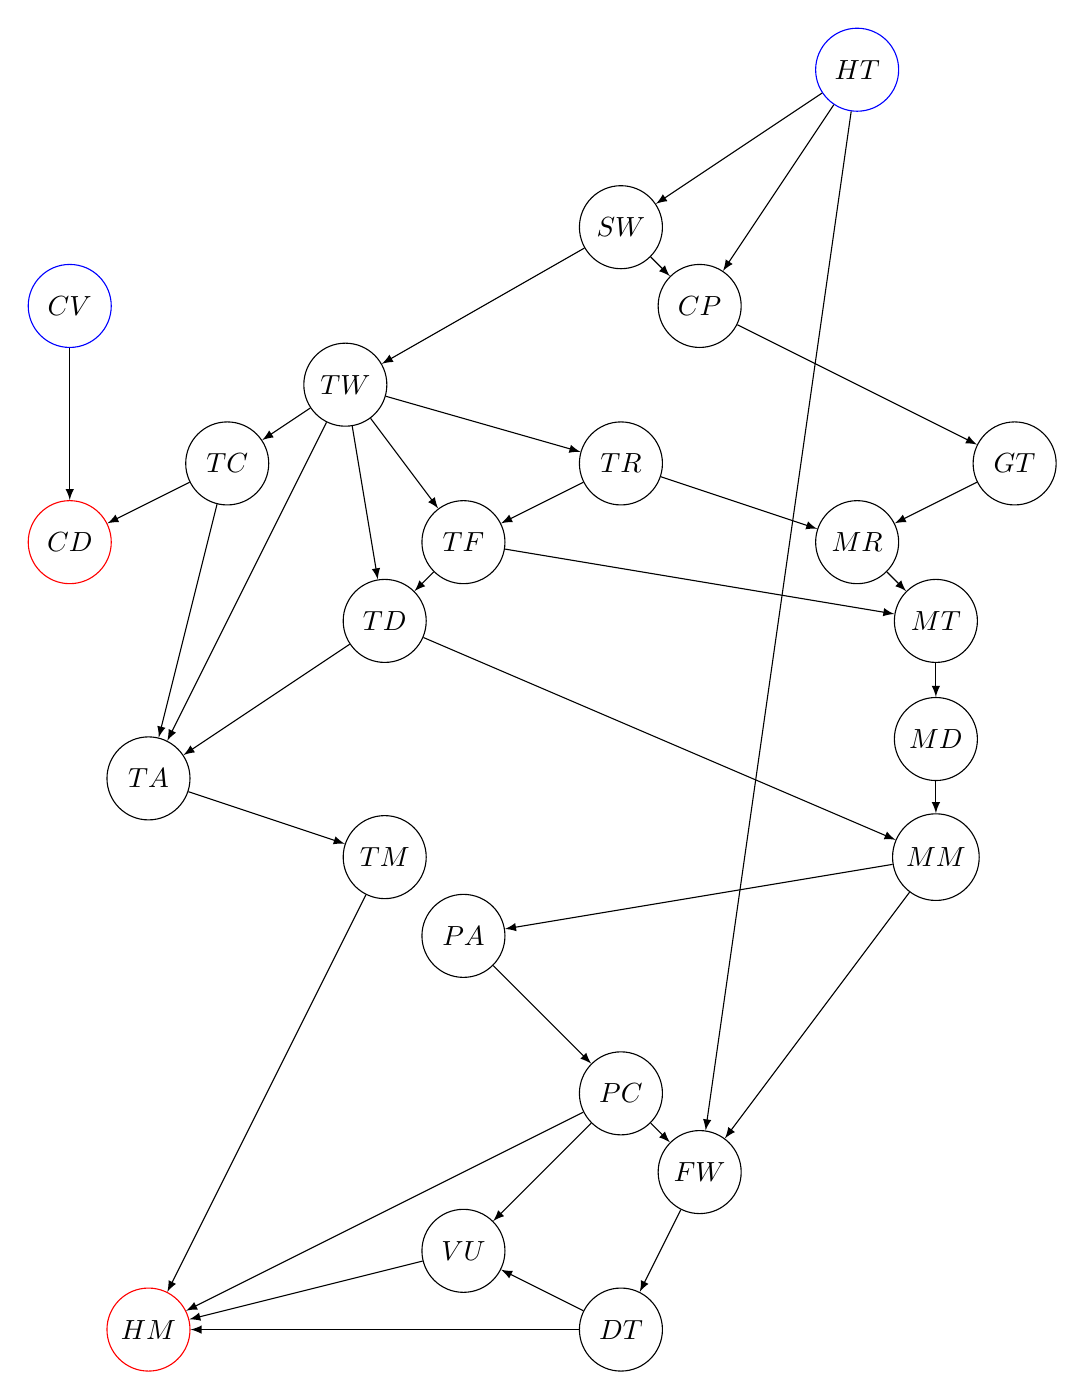
\begin{tikzpicture}
%     \begin{comment}
%     \node[circle,minimum width =30pt ,minimum height =30pt ,draw=blue] (1) at(4,16){$CV$};
% \node[circle,minimum width =30pt ,minimum height =30pt ,draw=blue] (2) at(14,19){$HT$};
% \node[circle,minimum width =30pt ,minimum height =30pt ,draw=blue] (3) at(11,17){$SW$};
% \node[circle,minimum width =30pt ,minimum height =30pt ,draw=blue] (4) at(7.5,15){$TW$};
% \node[circle,minimum width =30pt ,minimum height =30pt ,draw=blue] (5) at(6,14){$TC$};
% \node[circle,minimum width =30pt ,minimum height =30pt ,draw=blue] (6) at(4,13){$CD$};
% \node[circle,minimum width =30pt ,minimum height =30pt ,draw=blue] (7) at(11,14){$TR$};
% \node[circle,minimum width =30pt ,minimum height =30pt ,draw=blue] (8) at(9,13){$TF$};
% \node[circle,minimum width =30pt ,minimum height =30pt ,draw=blue] (9) at(8,12){$TD$};
% \node[circle,minimum width =30pt ,minimum height =30pt ,draw=blue] (10) at(5,10){$TA $};
% \node[circle,minimum width =30pt ,minimum height =30pt ,draw=blue] (11) at(8,9){$TM$};
% \node[circle,minimum width =30pt ,minimum height =30pt ,draw=blue] (12) at(12,16){$CP$};
% \node[circle,minimum width =30pt ,minimum height =30pt ,draw=blue] (13) at(16,14){$GT$};
% \node[circle,minimum width =30pt ,minimum height =30pt ,draw=blue] (14) at(14,13){$MR$};
% \node[circle,minimum width =30pt ,minimum height =30pt ,draw=blue] (15) at(15,12){$MT$};
% \node[circle,minimum width =30pt ,minimum height =30pt ,draw=blue] (16) at(15,10.5){$MD$};
% \node[circle,minimum width =30pt ,minimum height =30pt ,draw=blue] (17) at(15,9){$MM $};
% \node[circle,minimum width =30pt ,minimum height =30pt ,draw=blue] (18) at(9,8){$PA$};
% \node[circle,minimum width =30pt ,minimum height =30pt ,draw=blue] (19) at(11,6){$PC$};
% \node[circle,minimum width =30pt ,minimum height =30pt ,draw=blue] (20) at(12,5){$FW$};
% \node[circle,minimum width =30pt ,minimum height =30pt ,draw=blue] (21) at(11,3){$DT$};
% \node[circle,minimum width =30pt ,minimum height =30pt ,draw=blue] (22) at(9,4){$VU$};
% \node[circle,minimum width =30pt ,minimum height =30pt ,draw=blue] (23) at(5,3){$HM$};
%     \end{comment}

\node[circle,minimum width =30pt ,minimum height =30pt ,draw=blue] (1) at(4,16){$CV$};
\node[circle,minimum width =30pt ,minimum height =30pt ,draw=blue] (2) at(14,19){$HT$};
\node[circle,minimum width =30pt ,minimum height =30pt ,draw=black] (3) at(11,17){$SW$};
\node[circle,minimum width =30pt ,minimum height =30pt ,draw=black] (4) at(7.5,15){$TW$};
\node[circle,minimum width =30pt ,minimum height =30pt ,draw=black] (5) at(6,14){$TC$};
\node[circle,minimum width =30pt ,minimum height =30pt ,draw=red] (6) at(4,13){$CD$};
\node[circle,minimum width =30pt ,minimum height =30pt ,draw=black] (7) at(11,14){$TR$};
\node[circle,minimum width =30pt ,minimum height =30pt ,draw=black] (8) at(9,13){$TF$};
\node[circle,minimum width =30pt ,minimum height =30pt ,draw=black] (9) at(8,12){$TD$};
\node[circle,minimum width =30pt ,minimum height =30pt ,draw=black] (10) at(5,10){$TA $};
\node[circle,minimum width =30pt ,minimum height =30pt ,draw=black] (11) at(8,9){$TM$};
\node[circle,minimum width =30pt ,minimum height =30pt ,draw=black] (12) at(12,16){$CP$};
\node[circle,minimum width =30pt ,minimum height =30pt ,draw=black] (13) at(16,14){$GT$};
\node[circle,minimum width =30pt ,minimum height =30pt ,draw=black] (14) at(14,13){$MR$};
\node[circle,minimum width =30pt ,minimum height =30pt ,draw=black] (15) at(15,12){$MT$};
\node[circle,minimum width =30pt ,minimum height =30pt ,draw=black] (16) at(15,10.5){$MD$};
\node[circle,minimum width =30pt ,minimum height =30pt ,draw=black] (17) at(15,9){$MM $};
\node[circle,minimum width =30pt ,minimum height =30pt ,draw=black] (18) at(9,8){$PA$};
\node[circle,minimum width =30pt ,minimum height =30pt ,draw=black] (19) at(11,6){$PC$};
\node[circle,minimum width =30pt ,minimum height =30pt ,draw=black] (20) at(12,5){$FW$};
\node[circle,minimum width =30pt ,minimum height =30pt ,draw=black] (21) at(11,3){$DT$};
\node[circle,minimum width =30pt ,minimum height =30pt ,draw=black] (22) at(9,4){$VU$};
\node[circle,minimum width =30pt ,minimum height =30pt ,draw=red] (23) at(5,3){$HM$};

    \draw[->] (1) --(6);
\draw[->] (2) --(3);
\draw[->] (2) --(12);
\draw[->] (2) --(20);
\draw[->] (3) --(4);
\draw[->] (3) --(12);
\draw[->] (4) --(5);
\draw[->] (4) --(7);
\draw[->] (4) --(8);
\draw[->] (4) --(9);
\draw[->] (4) --(10);
\draw[->] (5) --(6);
\draw[->] (5) --(10);
\draw[->] (7) --(8);
\draw[->] (7) --(14);
\draw[->] (8) --(9);
\draw[->] (8) --(15);
\draw[->] (9) --(10);
\draw[->] (9) --(17);
\draw[->] (10) --(11);
\draw[->] (11) --(23);
\draw[->] (12) --(13);
\draw[->] (13) --(14);
\draw[->] (14) --(15);
\draw[->] (15) --(16);
\draw[->] (16) --(17);
\draw[->] (17) --(18);
\draw[->] (17) --(20);
\draw[->] (18) --(19);
\draw[->] (19) --(20);
\draw[->] (19) --(22);
\draw[->] (19) --(23);
\draw[->] (20) --(21);
\draw[->] (21) --(22);
\draw[->] (21) --(23);
\draw[->] (22) --(23);


\end{tikzpicture}

